\section{LIMDD}


\begin{frame}
\begin{refsection}

\vfill
	
	\centering
	\textbf{\Large Stabilizer Formalism, Decision Diagrams and \limdd~\cite{vinkhuijzen2021limdd}}
	
	
\vfill

\printbibliography[section=\therefsection]
\end{refsection}

\end{frame}




\begin{frame}{Quantum State Representation with the
					\alert{Stabilizer Formalism}}


\begin{definition}
Stabilizer States are:

\begin{itemize} 
	\item
A non-universal subset of all quantum states crucial for error correction, etc: 

\begin{center}
\begin{tikzpicture}\footnotesize
  \tikzset{venn circle/.style={circle,minimum width=2cm,fill=####1,opacity=0.4}}
  \node [venn circle=white,minimum width=2.5cm,draw] (A) at (0,0.3) {};
  \node  at (0,1.25) 			{State space};

%  \node [venn circle = Red!40!white, ellipse,minimum height=2.2cm, minimum width=3.6cm] (L) at (0,0.6) {};
%  \node  at (0,1.5) 		{\limdd};
  
%  \node [venn circle = blue!70!white,text width=1.3cm,align=center,rotate=79,ellipse,minimum height=1.8cm, minimum width=2.5cm] (B) at (-.6,-.2) {};
%  \node[text width=1.3cm,align=center]  at (-.9,-1.) {MPS};


%  \node [venn circle = green!70!white,text width=1.3cm,align=center,rotate=119,ellipse,minimum height=1.8cm, minimum width=2.5cm] (B) at (.6,-.2) {};
%  \node[text width=1.3cm,align=center]  at (.9,-1.) {RBM};



%  \node [venn circle = Blue!100!white,text width=1cm,align=center, minimum width=1.cm] (B) at (-.5,.3) 	{\textcolor{white}{QMDD}};						

  \node [venn circle = OliveGreen,text width=1cm,align=center, minimum width=1.cm,opacity=.5,text opacity=1] (C) at (.5,.2) {\textcolor{white}{Stabilizer states}};
\end{tikzpicture}					
\end{center}

\pause

\item A stabilizer state $\ket{\phi}$ is uniquely defined by 
			$n$-qubit Pauli operators ($n \times$):
\[
\left\{
\begin{matrix}
\pm P_{1,1}~~~ \otimes & P_{1,2}~~~ \otimes & \dots & \otimes~~~ P_{1,n},\\
\pm P_{2,1}~~~ \otimes& P_{2,2}~~~  \otimes& \dots & \otimes~~~ P_{2,n},\\
\vdots  & \vdots  & \ddots& \vdots\\
\pm P_{n,1}~~~ \otimes& P_{n,2}~~~ \otimes & \dots &  \otimes~~~ P_{n,n},\\
\end{matrix} 
\right\}
\text{ for } P_{i,j} \in \hspace{-.5em} \underbrace{\set{\id, X, Y, Z}}_{ \text{ single qubit Pauli's}}
\]	
\pause

with $P_{i,1} \otimes  P_{i,2} \otimes  \dots  \otimes P_{i,n} \cdot \ket{\phi} = \ket{\phi}$ (state $\ket{\phi}$ is stabilized by each Pauli op.)

\pause

\item Closed under the stabilizer (or Clifford) gate set: \set{S, H, CNOT}

\item Efficiently classically simulatable!
\pause
\item \alert{Used in error correction, quantum networking, etc etc.}
\end{itemize}
\end{definition}



\end{frame}




\begin{frame}{Quantum State Representation with the
					\alert{Stabilizer Formalism}}


\vspace{-.5em}
Pauli gates:~~~~ $I = \mat{1&0\\0&1},~~~~X = \mat{0&1\\1&0} ~~~~Y = \mat{0&-i\\i&0}~~~~Z = \mat{1&0\\0&-1}$


\begin{exampleblock}{Two-qubit stabilizer states}

\begin{itemize}
\item ~~$Z \cdot \ket{0} = \mat{1&0\\0&-1} \cdot \mat{1\\0} = \mat{1\\0} = \ket 0$
\item $-Z \cdot \ket{1} = \mat{-1&0\\0&1} \cdot \mat{0\\1} = \mat{0\\1} = \ket 1$
\pause
\item
\only<+>{ ~~$P \cdot \ket{+} = ~~P \cdot \mat{1\\1} = \mat{1\\1} = \ket +$ for which $P \in \set{\mathbb{I}, X, Y, Z}$?}
\pause
 ~~$X \cdot \ket{+} = ~~X \cdot \mat{1\\1} = \mat{1\\1} = \ket +$, etc
%\pause
%\item
% $-X \cdot \ket{-} = ~~X \cdot \mat{1\\1} = \mat{1\\1} = \ket -$ 
\pause
\vspace{-.5em}
	\item The computational basis state $\ket{00}$ is stabilized by $\left\{\amat{Z\otimes I,\\ I\otimes Z\phantom,}\right\}$
	\item The Bell state $
    \ket{\Phi} \approx  \ket{00} + \ket{11}
$ is stabilized by $\left\{\amat{Z\otimes Z,\\ X\otimes X\phantom,}\right\}$, \pause e.g., $X\otimes X \cdot \ket{\Phi} = \ket{\Phi}$
\end{itemize}

%\vspace{.5em}

%Indeed, we have 
% and $Z\otimes Z \cdot \ket{\Phi} = \ket{\Phi}$.


\pause

\vspace{.5em}

We can apply gate $H $ to qubit two of $\ket{\Phi}$ as follows:
\vspace{.5em}

\centering
$\left\{\amat{Z\otimes Z,\\ X\otimes X\phantom,}\right\} \underrightarrow{~~~~~~I \otimes H~~~~~~~~}
\left\{\amat{Z\otimes \alert{X},\\ X\otimes \alert{Z}\phantom,}\right\} 
$

%\begin{columns}
%\begin{column}{.3\textwidth}
%~~~~~~~The Bell state:\\
%~~~~~~$
%    \ket{\phi} \approx  \ket{00} + \ket{11}
%%    \begin{bmatrix*}[c]
%%    1,\\ 0,\\ 0,\\ 1\phantom,\\
%%    \end{bmatrix*}
%$
%\end{column}
%\begin{column}{.18\textwidth}
%\Qcircuit @C=2.3em @R=1.2em {
% & \gate{X} & \qw  \\
%&  \gate{X} & \qw \\ 
%  & \lstick{X \otimes X\hspace{-1cm}} & \dstick{}
%\gategroup{1}{2}{2}{2}{.7em}{--}
%}
%\end{column}
%\begin{column}{.18\textwidth}
%\Qcircuit @C=2.3em @R=1.2em {
% & \gate{Z} & \qw  \\
%&  \gate{Z} & \qw \\
%  & \lstick{Z\otimes Z\hspace{-1cm}} & \dstick{}
%\gategroup{1}{2}{2}{2}{.7em}{--}
%}
%\end{column}
%\begin{column}{.3\textwidth}
%Stabilized by:
%\vspace{3mm}
%
%$
%\ket{\phi} = X \otimes X \cdot \ket { \phi }
%$
%
%$
%\ket{\phi} = Z \otimes Z \cdot \ket { \phi }
%$
%\end{column}
%\end{columns}

\end{exampleblock}

\vspace{-.5em}
\pause

\begin{alertblock}{Caveats}
	
\vspace{-.5em}
\begin{itemize}
\item The stabilizer formalism is non-universal, \hfill but  important and tractable
\item The stabilizer tableau uniquely defines a state, \hfill but many tableaux do as well
%\item Classical simulation is tractable, \hfill but non-universal (as expected)\\
\end{itemize}
\vspace{-.5em}

\end{alertblock}


				
\end{frame}	






\begin{frame}[fragile]{Quantum State Representation with
					\alert{Decision Diagrams}}

\vspace{-1em}
We can think of a quantum state $\ket{\phi}$ as a pseudo Boolean function $f \colon \set{0,1}^n \to \complex$, or

\begin{block}{`Shannon decomposition' in quantum}

\centering

\vspace{.5em}

\scalebox{1.2}{
$\ket{\phi} = \ket 0 \otimes \hspace{-1em} \underbrace{\ket{\phi_0}}_{\text{$n-1$ qubits}} + ~~~~
			 \ket 1  \otimes \hspace{-1em} \underbrace{\ket{\phi_1}}_{\text{$n-1$ qubits}}$
}

\vspace{.5em}

\scalebox{1.2}{
~~~~~~~~~~~~~~~~~$\ket{\phi} = \alpha_1 \ket{00\dots00}  + \dots  + \alpha_{2^n} \ket{11\dots11} $

}\hfill (recursively)

\vspace{.5em}
\end{block}

%\begin{block}{View quantum state as pseudo Boolean function}
%
%A state is an amplitude function
%\scalebox{1.2}{
%$ f \colon \bool^n \to \complex $
%} with
%\scalebox{1.2}{
%$\ket{\phi} = \displaystyle \sum_{i \in \bool^n} f(i) \ket{i}$.
%}
%\end{block}
%
%
%\begin{textblock}{14}(0,.3)
%\centering
%\only<1>{
%\tikzset{every picture/.style={->,thick}}
%%~\hspace{-.6cm}
%\begin{tikzpicture}[
%    scale=0.3,
%    every path/.style={>=latex},
%    every node/.style={},
%    inner sep=0pt,
%    minimum size=0.3cm,
%    line width=1pt,
%    node distance=1cm,
%    thick,
%    font=\footnotesize
%    ]
%\node[] (vec) {
%    \begin{minipage}{2cm}\footnotesize
%    $
%	\def\arraystretch{1.3}
%    \begin{matrix*}[c]
%    f_{000}=\\f_{001}=\\f_{010}=\\f_{011}=\\f_{100}=\\f_{101}=\\f_{110}=\\f_{111}=\\
%    \end{matrix*}
%    \begin{bmatrix*}[c]
%    1, \\0, \\ 2,\\ 0, \\ 1,\\ 0, \\ -2,\\0\phantom{,}\\
%    \end{bmatrix*}
%	\begin{minipage}{1cm}
%	$\left.
%    \begin{matrix}
%      \\ \\ \\ \\
%    \end{matrix}
%\~~\right \}{= f_0}\\
%    \begin{matrix}
%      \\ \\ \\ \\
%    \end{matrix}
%    $
%	\end{minipage}
%    $
%    \end{minipage}
%};
%\end{tikzpicture}
%}
%\end{textblock}
%
%
\pause


\tikzset{every picture/.style={->,thick}}
~\hspace{-1cm}
\begin{tikzpicture}[
    scale=0.3,
    every path/.style={>=latex},
    every node/.style={},
    inner sep=0pt,
    minimum size=0.3cm,
    line width=1pt,
    node distance=1cm,
    thick,
    font=\footnotesize
    ]



    % nodes    
    \node[draw,circle] (a1) {};
    \node[draw,circle, below = .45cm of a1, xshift=-.9cm] (a2) {};
    \node[draw,circle, below = .45cm of a1, xshift= .9cm] (a3) {};
    \node[draw,circle, below = .45cm of a2, xshift=-.3cm] (a41) {};
    \draw[e0=  0] (a2) edge  node[] {} (a41);

    \node[draw,circle, below = .45cm of a2, xshift= .3cm] (a42) {};
    \node[draw,circle, below = .45cm of a3, xshift=-.3cm] (a43) {};
    \node[draw,circle, below = .45cm of a3, xshift= .3cm] (a44) {};
    \node[leaf, below=.45cm of a41, xshift=-.5cm      ] (w1) {$1$};
    \draw[e0=  0] (a41) edge  node[] {} (w1);

\onslide<2>{
    \node[leaf, right= .02cm of w1,inner sep=0pt] (w2) {$0$};
    \draw[e1=  0] (a41) edge  node[] {} (w2);
}
    \node[leaf, right= .04cm of w2,inner sep=0pt] (w3) {$2$};
\onslide<2>{
    \node[leaf, right= .02cm of w3,inner sep=0pt] (w4) {$0$};
    \draw[e1=  0] (a42) edge  node[] {} (w4);
}
    \node[leaf, right= .02cm of w4,inner sep=0pt] (w5) {$1$};
\onslide<2>{
    \node[leaf, right= .02cm of w5,inner sep=0pt] (w6) {$0$};
    \draw[e1=  0] (a43) edge  node[] {} (w6);
}
    \node[leaf, right= .02cm of w6,inner sep=0pt] (w7) {$-2$};
\onslide<2>{
    \node[leaf, right= .02cm of w7,inner sep=0pt] (w8) {$0$};
    \draw[e1=  0] (a44) edge  node[] {} (w8);
}
        
    % edges
    \draw[<-] (a1) --++(90:2cm) node[right,pos=.7] {};
    \draw[e0 = 0] (a1) edge  node[] {} (a2);
    \draw[e1 = 0] (a1) edge  node[] {} (a3);

    \draw[e1=  0] (a2) edge  node[] {} (a42);
    \draw[e0=  0] (a3) edge  node[] {} (a43);
    \draw[e1=  0] (a3) edge  node[] {} (a44);
    \draw[e0=  0] (a42) edge  node[] {} (w3);
    \draw[e0=  0] (a43) edge  node[] {} (w5);
    \draw[e0=  0] (a44) edge  node[] {} (w7);




\node[left = 1.3cm of a1.south,yshift=-1cm] (vec) {
    \begin{minipage}{1.7cm}\footnotesize
    $
%\frac 12\cdot
\def\arraystretch{1.3}
    \begin{bmatrix*}[r]
			 \only<4->{\color{red} 1}\only<-3>{1}\\\only<4->{\color{red} 0}\only<-3>{0}\\
    		 \only<7->{\color{purple} 2}\only<-6>{2}\\\only<7->{\color{purple} 0}\only<-6>{0}\\
    		\only<4->{\color{green} 1}\only<-3>{1}\\\only<4->{\color{green} 0}\only<-3>{0}\\ 
    		\only<7->{\color{blue}-2}\only<-6>{-2}\\
    		\only<7->{\color{blue} 0}\only<-6>{0} \\
    \end{bmatrix*}$
    \end{minipage}
};


    \node[below= 2.5cm of a1]   (dt)  {Decision tree};



\pause


\pause


    \node[draw,circle, below = .45cm of a2, xshift=-.3cm,fill=red] (a41) {};
%    \node[draw,circle, below = .45cm of a2, xshift= .3cm,fill=purple] (a42) {};
    \node[draw,circle, below = .45cm of a3, xshift=-.3cm,fill=green] (a43) {};
%    \node[draw,circle, below = .45cm of a3, xshift= .3cm,fill=blue] (a44) {};

\only<4>{
\node[right= of a1, text width = 3cm] {
\color{red}$f_{00} = \begin{bmatrix*}[c]
    				   1 \\ 0\\
    				\end{bmatrix*}$\\\vspace{3mm}
\color{green}\scriptsize$ f_{10} = f_{00}$\\\vspace{4mm}
};
}


\pause

    % nodes
    \node[draw,circle, right= 3.5cm of a1] (a1) {};
    \node[draw,circle, below = .45cm of a1, xshift=-.9cm] (a2) {};
    \node[draw,circle, below = .45cm of a1, xshift= .9cm] (a3) {};
%    \node[draw,circle, below = .45cm of a2, xshift=-.3cm] (a41) {};
    \node[draw,circle, below = .45cm of a2, xshift= .3cm] (a42) {};
    \node[draw,circle, below = .45cm of a3, xshift=-.3cm,shade, shading=axis, left color=red,  right color=green, shading angle=90] (a43) {};
    \node[draw,circle, below = .45cm of a3, xshift= .3cm] (a44) {};

\only<-5>{
    \node[leaf, below= .45cm of a42, xshift= -.13cm, inner sep=0pt] (w3) {$2$};
	\onslide<2>{
    \node[leaf, right= .02cm of w3,inner sep=0pt] (w4) {$0$};
	}
    \node[leaf, right= .02cm of w4,inner sep=0pt] (w5) {$1$};
	\onslide<2>{
    \node[leaf, right= .02cm of w5,inner sep=0pt] (w6) {$0$};
	}
    \node[leaf, right= .02cm of w6,inner sep=0pt] (w7) {$-2$};

    \draw[e0= 0] (a42) edge   (w3);
    \draw[e0= 0] (a43) edge   (w5);
    \draw[e0= 0] (a44) edge  (w7);
}

\only<6->{
    \node[leaf, below= .45cm of a42, xshift=.6cm] (w1) {$1$};
    
    \draw[e0= 0] (a42) edge  node[above right,pos=.3] {$2$} (w1);
    \draw[e0= 0] (a43) edge  node[above left,pos=.3] {} (w1);
    \draw[e0=-20] (a44) edge  node[pos=.4,below right] {$-2$} (w1);
}


    % edges
    \draw[<-] (a1) --++(90:2cm) node[right,pos=.7] {};
    \draw[e0 = 0] (a1) edge  node[] {} (a2);
    \draw[e1 = 0] (a1) edge  node[] {} (a3);

    \draw[e0=  0] (a2) edge  node[] {} (a43);
    \draw[e1=  0] (a2) edge  node[] {} (a42);
    \draw[e0=  0] (a3) edge  node[] {} (a43);
    \draw[e1=  0] (a3) edge  node[] {} (a44);

    

    \node[below= 2.5cm of a1]  (add)   {Algebraic DD (ADD)};


\pause
\pause

%    \node[draw,circle, below = .45cm of a2, xshift=-.3cm,fill=red] (a41) {};
    \node[draw,circle, below = .45cm of a2, xshift= .3cm,fill=purple] (a42) {};
    \node[draw,circle, below = .45cm of a3, xshift=-.3cm,fill=green] (a43) {};
    \node[draw,circle, below = .45cm of a3, xshift= .3cm,fill=blue] (a44) {};

\only<7>{
\node[right= of a3, text width = 3cm] {
\color{green}$f_{00} = f_{10} = \begin{bmatrix*}[c]
    				   1, \\ 0\phantom{,}\\
    				\end{bmatrix*}$\\\vspace{4mm}
\color{purple}\scriptsize$f_{01}  =\phantom-2\cdot  f_{00}$\\\vspace{4mm}
%\color{green}\scriptsize$ f_{10} = \phantom-2\cdot  f_{00}$\\\vspace{4mm}
\color{blue}\scriptsize$f_{11}=-2 \cdot f_{00}$
};
}


\pause


    % nodes
    \node[draw,circle, right= 2.8cm of a1] (a1) {};
    \node[draw,circle, below = .45cm of a1, xshift=-.7cm] (a2) {};
    \node[draw,circle, below = .45cm of a1, xshift= .7cm] (a3) {};
    \node[draw,circle, below = .45cm of a2, xshift= .7cm,shade, shading=axis, left color=purple,  middle color=purple, right color=blue, shading angle=90] (a41) {};
    \node[leaf, below= .45cm of a41] (w1) {$1$};

    
    % edges
    \draw[<-] (a1) --++(90:2cm) node[right,pos=.7] {};
    \draw[e0 = 0] (a1) edge  node[] {} (a2);
    \draw[e1 = 0] (a1) edge  node[] {} (a3);

    \draw[e0= 20] (a2) edge  node[left,pos=.4] {} (a41);
    \draw[e1= 20] (a2) edge  node[above right,pos=.3] {~$2$} (a41);
    \draw[e0= 20] (a3) edge  node[left,pos=.] {} (a41);
    \draw[e1= 20] (a3) edge  node[right,pos=.4] {$-2$} (a41);
    \draw[e0=0] (a41) edge  node[left] {} (w1);
%    \draw[e1=25] (a41) edge  node[lbl,right] {$0$} (w1);

\node[below= 2.5cm of a1] (aadd) {QMDD};


\pause

\node[below= .3cm of dt, xshift=-2cm] {\alert{\textbf{Merge nodes $v, w$: }}};
\node[below= .3cm of dt] {\alert{~~~~Never}};
\node[below= .3cm of add] {\alert{$\ket v = \ket w$ }};
\node[below= .3cm of aadd, xshift=.cm,text width = 4cm,align=center] {\alert{$\ket v = \gamma \cdot \ket w$\\ \vspace{3mm}(equivalent up to a complex factor $\lambda$)}};

    \onslide<1->
\end{tikzpicture}

\pause
\centering
\alert{(QMDD can be exponentially more succinct than ADD.)}


\end{frame}


%\end{comment}



\begin{frame}{Benefits of \ul{Decision Diagrams}}

\begin{block}{Why Decision Diagrams?}
\begin{itemize}
	\item Succinct representation of many quantum states: 
		\alert{\#nodes $\ll 2^n$}\\
		(Empirical results show circuit simulation up to 70 qubits.)
	\item<2-> ``Homomorphic compression scheme'' for combinatorial data
	\item<5-> Operations often linear-time in the size of the DD: 
%	(\alert{number of nodes $m$}):
	\\
		\centering
		\vspace{2mm}
\phantom{ZZZZZZZZZZ}		\scalebox{1.2}{
$
 \ket{\underbrace{\phi_{i+1}}_{
\oh(\alert m)}} ~~=~~ \underbrace{U_1}_{\oh(1)} ~~\cdot~~ \ket{\underbrace{{\phi_i}}_{\hspace{5mm}\alert m ~\ll~ 2^n\hspace{-2mm}}}
$
}
\end{itemize}
\end{block}


\vfill

\pause
\pause


\begin{exampleblock}{Simulation is (often simpler than) matrix-vector multiplication}
\begin{columns}
\begin{column}{.3\textwidth}
~~~~~~\Qcircuit @C=2.3em @R=1.2em {
 & \gate{X} & \qw  \\
& \qw      & \qw \\% \lstick{\phi_1} \\
& \qw      & \qw \\
  & \dstick{X \otimes I \cdot \ket{\phi_i} = \ket{\phi_{i+1}}} & \dstick{}
\gategroup{1}{2}{3}{2}{.7em}{--}
}

~\\

~\\
\end{column}
\begin{column}{.7\textwidth}
	
	\tikzset{every picture/.style={->,thick}}
~\hspace{-1cm}
\begin{tikzpicture}[
    scale=0.3,
    every path/.style={>=latex},
    every node/.style={},
    inner sep=0pt,
    minimum size=0.3cm,
    line width=1pt,
    node distance=1cm,
    thick,
    font=\footnotesize
    ]



\node[] (vec) {
    \begin{minipage}{3.4cm}\footnotesize
    $
X \otimes I \cdot
\def\arraystretch{1.3}
    \begin{bmatrix*}[c]
    \color{red} 1 \\\color{red}{0} \\ 
    \color{red}{2}\\\color{red}{0}\\
    \color{green}    		{1}\\
    \color{green}{0}\\ 
    \color{green}{-2}\\
    \color{green}{0} \\
    \end{bmatrix*}
    ~~~=~~~
    \begin{bmatrix*}[c]
    \color{green}    		{1}\\\color{green}{0}\\ 
    		\color{green}{-2}\\\color{green}{0{}} \\
    \color{red}{1} \\\color{red}{0} \\ \color{red}{2}\\\color{red}{0}\\
    \end{bmatrix*}
    $
    \end{minipage}
};

\pause
    % nodes
    \node[draw,circle, right= .8cm of vec,yshift=1cm] (a1) {};
    \node[draw,circle, below = .45cm of a1, xshift=-.6cm,fill=red] (a2) {};
    \node[draw,circle, below = .45cm of a1, xshift= .6cm,fill=green] (a3) {};
    \node[draw,circle, below = .45cm of a2, xshift= .6cm] (a4) {};
    \node[draw,circle,rectangle,minimum size=0.4cm, below= .45cm of a4] (w1) {$1$};
    
    % edges
    \draw[<-] (a1) --++(90:2cm) node[,right=1mm,pos=.8] {\scalebox{1.4}{$\phi_i$}};
    \draw[e0] (a1) edge  node[,left,pos=.2] {} (a2);
    \draw[e1] (a1) edge  node[,right,pos=.2] {} (a3);


    \draw[e0= 20] (a2) edge  node[] {} (a4);
    \draw[e1= 20] (a2) edge  node[above right,pos=.3] {$2$} (a4);
    \draw[e0= 20] (a3) edge  node[] {} (a4);
    \draw[e1= 20] (a3) edge  node[right] {$-2$} (a4);
    \draw[e0= 0] (a4) edge  node[] {} (w1);
%    \draw[e1= 25] (a4) edge  node[lbl,right] {$0$} (w1);
    
    
    \node[right= .5mm of a3] {\scalebox{1.3}{$\underrightarrow{~~X \otimes I~~}$}};

    % nodes
    \node[draw,circle, right= 3.6cm of vec,yshift=1cm] (a1) {};
    \node[draw,circle, below = .45cm of a1, xshift=-.6cm,fill=red] (a2) {};
    \node[draw,circle, below = .45cm of a1, xshift= .6cm,fill=green] (a3) {};
    \node[draw,circle, below = .45cm of a2, xshift= .6cm] (a4) {};
    \node[draw,circle,rectangle,minimum size=0.4cm, below= .45cm of a4] (w1) {$1$};
    
    % edges
    \draw[<-] (a1) --++(90:2cm) node[,right=1mm,pos=.8] {\scalebox{1.4}{$\phi_{i+1}$}};
    \draw[color=orange,e1] (a1) edge  node[left,pos=.2] {} (a2);
    \draw[color=orange,e0] (a1) edge  node[right,pos=.2] {} (a3);

    \draw[e0= 20] (a2) edge  node[] {} (a4);
    \draw[e1= 20] (a2) edge  node[above right,pos=.3] {$2$} (a4);
    \draw[e0= 20] (a3) edge  node[] {} (a4);
    \draw[e1= 20] (a3) edge  node[right] {$-2$} (a4);
    \draw[e0= 0] (a4) edge  node[] {} (w1);
%    \draw[e1= 25] (a4) edge  node[lbl,right] {$0$} (w1);
    
    
    
\end{tikzpicture}
	
	
\end{column}
\end{columns}
\end{exampleblock}




\end{frame}



\begin{frame}[fragile]{Limitations of Decision Diagrams}


%\begin{center}
%\begin{tikzpicture}\footnotesize
%%  \tikzset{venn circle/.style={circle,minimum width=2cm,fill=####1,opacity=0.4}}
%  \node [venn circle=white,minimum width=2.5cm,draw] (A) at (0,0.3) {};
%  \node  at (0,1.25) 			{State space};
%
%%  \node [venn circle = Red!40!white, ellipse,minimum height=2.2cm, minimum width=3.6cm] (L) at (0,0.6) {};
%%  \node  at (0,1.5) 		{\limdd};
%  
%%  \node [venn circle = blue!70!white,text width=1.3cm,align=center,rotate=79,ellipse,minimum height=1.8cm, minimum width=2.5cm] (B) at (-.6,-.2) {};
%%  \node[text width=1.3cm,align=center]  at (-.9,-1.) {MPS};
%
%
%%  \node [venn circle = green!70!white,text width=1.3cm,align=center,rotate=119,ellipse,minimum height=1.8cm, minimum width=2.5cm] (B) at (.6,-.2) {};
%%  \node[text width=1.3cm,align=center]  at (.9,-1.) {RBM};
%
%
%  \node [venn circle = Blue!100!white,text width=1cm,align=center, minimum width=1.cm] (B) at (-.5,.3) 	{\textcolor{white}{poly-QMDD}};						
%
%  \node [venn circle = OliveGreen,text width=1cm,align=center, minimum width=1.cm,opacity=.5,text opacity=1] (C) at (.5,.2) {\textcolor{white}{Stabilizer states}};
%\end{tikzpicture}					
%\end{center}

\begin{alertblock}{QMDD can't succinctly represent stabilizer states, yet:}
	\begin{itemize}
%		\item For \alert{stabilizer states}, we proved  that QMDD can be exponential
		\item Stabilizers are a subset of states that are \alert{classically simulatable!}
		\item Important in error correction, measurement-based QC and circuit equivalence
	\end{itemize}
\end{alertblock}


\begin{theorem}%[\cite{vinkhuijzen2021limdd} ]
QMDD requires $2^\Omega({\sqrt{n}})$ space to represent 
	$\sqrt n\times \sqrt n$ grid graph states.
\end{theorem}


\begin{refsection}

\vfill

\newcommand{\swl}[2][nmbr]{\eqmakebox[#1]{\strut #2}}

\vspace{-.9cm}

\pause

\hspace{-.5cm}
\begin{minipage}{4cm}
\[
\left\{
\begin{matrix}
\swl I \otimes  \swl Z \otimes \dots \otimes \swl I \otimes Z,\\
\swl I \otimes I  \otimes  \dots \otimes Z\otimes  \swl I,\\
\swl \vdots \phantom{\otimes}  \ddots  \phantom{\dots} \phantom{\otimes} \phantom{\otimes}  \phantom{\otimes}   \vdots,\\
\swl I  \otimes\swl  I \otimes  \dots \otimes \swl  I \otimes Z,\\
\swl I \otimes \swl I \otimes \dots \otimes  \swl I\otimes  \swl I\\
\end{matrix} 
\right\}
\]\vspace{2.2cm}
\end{minipage}
\scalebox{.5}{
    \vspace{-1cm}
    \begin{tikzpicture}[node distance=.2cm]
        \def\nx{3} \def\ny{3}
        \draw [black, ultra thick] (0,0) grid (\nx,\ny);
        \foreach \i in {0,...,\nx}
%    \pgfmathsetmacro\ii{\i / 2}
            \foreach \j in {0,...,\ny}
                \node[draw,fill=black,circle] at
                			  ({\i}, {\j}) {.};
                			  
    \node (b) at (3.6,.0) {};
    \node[above = 3cm of b] (t) {};
    \draw (b) edge[<->,ultra thick] node[right] {\Large $\sqrt n$} (t);
    
    \onslide<4->{	  
    \node (b) at (1.5,-1) {};
    \node[above = 4.5cm of b] (t) {};
    \draw (b) edge[ultra thick,color=red]  (t);
    }
    \end{tikzpicture}
}
\pause
\begin{tikzpicture}[
    scale=0.3,
    every path/.style={>=latex},
    every node/.style={},
    inner sep=0pt,
    minimum size=0.3cm,
    line width=1pt,
    node distance=.7cm,
    thick,
    font=\footnotesize
    ]
    
    % nodes    
    \node[draw,circle] (a1) {};

    \node[below = -.1cm of a1, xshift=-.9cm,text width=.2cm] (a2) {~\\~\\ \vdots};
    \node[below = -.1cm of a1, xshift= .9cm,text width=.2cm] (a3) {~\\~\\ \vdots};

    \node[below = -.21cm of a2, xshift=-.25cm] (a41) {};
    \node[ below = -.21cm of a2, xshift= .25cm] (a42) {};
    \node[ below = -.21cm of a3, xshift=-.25cm] (a43) {};
    \node[ below = -.21cm of a3, xshift= .25cm] (a44) {};


%    \draw[e0=  0] (a2) edge  node[] {} (a41);
    
    \node[draw,circle, below=.45cm of a41, xshift=-.5cm      ] (w1) {};
    \draw[e0=  0] (a41) edge  node[] {} (w1);

    \node[draw,circle, right= .12cm of w1,inner sep=0pt] (w2) {};
    \draw[e1=  0] (a41) edge  node[] {} (w2);

    \node[draw,circle, right= .12cm of w2,inner sep=0pt] (w3) {};

    \node[draw,circle, right= .12cm of w3,inner sep=0pt] (w4) {};
    \draw[e1=  0] (a42) edge  node[] {} (w4);

    \node[draw,circle, right= .12cm of w4,inner sep=0pt] (w5) {};

    \node[draw,circle, right= .12cm of w5,inner sep=0pt] (w6) {};
    \draw[e1=  0] (a43) edge  node[] {} (w6);

    \node[draw,circle, right= .12cm of w6,inner sep=0pt] (w7) {};

    \node[draw,circle, right= .12cm of w7,inner sep=0pt] (w8) {};
    \draw[e1=  0] (a44) edge  node[] {} (w8);


    \node[right = .2cm of w8,yshift=-.4cm] (b) {};
    \node[above = 2.1cm of b] (t) {};
    \draw (b) edge[<->] node[right] {$\nicefrac 12 n$} (t);

    % edges
    \draw[<-] (a1) --++(90:1.4cm) node[right,pos=.7] {};
    \draw[e0 = 0] (a1) edge  node[] {} (a2);
    \draw[e1 = 0] (a1) edge  node[] {} (a3);

    \draw[e0=  0] (a42) edge  node[] {} (w3);
    \draw[e0=  0] (a43) edge  node[] {} (w5);
    \draw[e0=  0] (a44) edge  node[] {} (w7);
    
    \draw [
    thick,
    decoration={
        brace,
        mirror,
        raise=0.1cm
    },
    decorate] (w1.south west) -- node[yshift=-.4cm] {\alert{unique sub-functions $f_{\vec c}$ for $\vec c\in \set{0,1}^{\nicefrac 12 n}$}} (w8.south east);
\end{tikzpicture}

\vspace{-2.5cm}

\begin{theorem}[\cite{lipton1979generalized}]
	A balanced bisection of the nodes of an $\sqrt n\times \sqrt n$ grid graph has $\Omega(\sqrt n)$ cross edges.
\end{theorem}



\printbibliography[section=\therefsection]
\end{refsection}

\end{frame}


\begin{frame}{\limdd Definition}

\begin{block}{Local-Invertible-Map DD (\limdd)}
\begin{itemize}
	\item A generalization of QMDD
	\item<2-> Nodes are merged up to $\gamma \cdot P_1 \otimes \dots \otimes P_n$ with $P_1, \dots, P_n \in \set{\id, X, Y, Z}$
%	\item<4-> All stabilizer states have linear \limdd size
%	\item<5-> Stabilizer (Clifford) circuit simulation is polynomial time in \limdd
\end{itemize}	
\end{block}


\pause
\pause

\begin{exampleblock}{\limdd example}
\centering

\scalebox{.9}{
\tikzset{every picture/.style={->,thick}}
~\hspace{-1cm}
\begin{tikzpicture}[
    scale=0.3,
    every path/.style={>=latex},
    every node/.style={},
    inner sep=0pt,
    minimum size=0.3cm,
    line width=1pt,
    node distance=1cm,
    thick,
    font=\footnotesize
    ]


\node[left = 1.cm of a1.south,yshift=-1cm] (vec) {
    \begin{minipage}{1.7cm}\footnotesize
    $
%\frac 12\cdot
\def\arraystretch{1.3}
    \begin{bmatrix*}[c]
			 {1,}\\{0,}\\
    		 {2,}\\{0,}\\
    		{1,}\\{0,}\\ 
    		{-2,}\\{0,\phantom{,}} \\
    \end{bmatrix*}$
    \end{minipage}
};


    % nodes
    \node[draw,circle, right= 1.8cm of vec,yshift=1cm] (a1) {};
    \node[draw,circle, below = .45cm of a1, xshift=-.7cm] (a2) {};
    \node[draw,circle, below = .45cm of a1, xshift= .7cm] (a3) {};
    \node[draw,circle, below = .45cm of a2, xshift= .7cm] (a4) {};
    \node[draw,circle,rectangle,minimum size=0.4cm, below= .45cm of a4] (w1) {$1$};
    
    % edges
    \draw[<-] (a1) --++(90:2cm) node[,right,pos=.8] {$f$};
    \draw[e0] (a1) edge  node[,left,pos=.2] {} (a2);
    \draw[e1] (a1) edge  node[,right,pos=.2] {} (a3);

    \draw[e0= 20] (a2) edge  node[] {} (a4);
    \draw[e1= 20] (a2) edge  node[above right,pos=.3] {$2$} (a4);
    \draw[e0= 20] (a3) edge  node[] {} (a4);
    \draw[e1= 20] (a3) edge  node[right] {$-2$} (a4);
    \draw[e0=  0] (a4) edge  node[] {} (w1);
%    \draw[e1= 25] (a4) edge  node[lbl,right] {$0$} (w1);
    
\node[below= 2.5cm of a1] (aadd) {QMDD};


    \node[right= .8cm of a3] {\scalebox{2.4}{$\rightsquigarrow$}};



    % nodes
    \node[draw,circle, right= 3.4cm of a1] (a1) {};
    \node[draw,circle, below = .45cm of a1] (a2) {};
%    \node[draw,circle, below = .45cm of a1, xshift= .7cm] (a3) {};
    \node[draw,circle, below = .45cm of a2] (a4) {};
    \node[draw,circle,rectangle,minimum size=0.4cm, below= .45cm of a4] (w1) {$1$};
    
    % edges
    \draw[<-] (a1) --++(90:2cm) node[,right,pos=.8] {$f$};
    \draw[e0=20] (a1) edge  node[,left,pos=.2] {} (a2);
    \draw[e1=20] (a1) edge  node[,right=2mm,pos=.2] {$ \alert{Z \otimes \id}$} (a2);

%    \draw[e1] (a1) edge  node[,right,pos=.2] {$2$} (a3);

    \draw[e0= 20] (a2) edge  node[] {} (a4);
    \draw[e1= 20] (a2) edge  node[above right,pos=.3] {~$2$} (a4);
    \draw[e0=  0] (a4) edge  node[] {} (w1);
%    \draw[e1= 25] (a4) edge  node[lbl,right] {$0$} (w1);
    
\node[below= 2.5cm of a1] (limdd) {\limdd};


\node[below= .2cm of aadd, xshift=-3cm,text width = 4cm] {{\textbf{Node merging strategy:} \\ \alert{(when do we merge  nodes $v,w$?)}}};
\node[below= .2cm of aadd, xshift=.cm,text width = 5.9cm,align=center] {\mbox{$\ket w = \gamma \cdot \ket v$}

 for \mbox{$\gamma \in \complex$}

 \vspace{1mm}\alert{(up to a complex factor)}};
\node[below= .2cm of limdd, xshift=.cm,text width = 4.9cm,align=center] {\mbox{$\ket w= \gamma  \cdot  P \cdot \ket v$}

for \mbox{$P \in \set{\id, X, Y ,Z}^{\otimes n}$}

\vspace{1mm}\alert{(up to a ``Pauli string'')}};
\end{tikzpicture}
}

\end{exampleblock}


\end{frame}



\begin{frame}{\limdds Definition}


\begin{block}{Local-Invertible-Map DD (\limdd)}
\begin{itemize}
	\item A generalization of QMDD
	\item Nodes are merged up to $\gamma \cdot P_1 \otimes \dots \otimes P_n$ with $P_1, \dots, P_n \in \set{\id, X, Y, Z}$
%	\item<+-> \limdd is small for stabilizer states (and beyond)
%	\item<+-> Stabilizer (Clifford) circuit simulation is polynomial time in \limdd
%	\item<+-> Qubic factor overhead in the number of qubits: $\times n^3$
\end{itemize}
\end{block}

\pause



\begin{theorem}%[\limdd~\cite{vinkhuijzen2021limdd}]
\limdd requires $O(n^2)$ space to represent any stabilizer state.
\end{theorem}

\centering
\scalebox{.9}{
\begin{tabular}{l|l|l|l|l}
    \begin{tikzpicture}[->,>=stealth',shorten >=1pt,auto,node distance=1cm,
        thick, state/.style={circle,draw,minimum size=0.5cm},font=\scriptsize, scale=0.3,
    inner sep=0pt,]       
 
    \node[state](1){};
    \node[leaf] (s)[below = .5cm of 1]{$1$};
        
    \draw[<-,e1] (1) --++(0:2.4cm) node[] {};
    
    \path[]
    (1)  edge[e0= 20]  node[pos=.6,left] {} (s)
    (1) edge[e1= 20]  node[pos=.45,] {} (s)
	;

\node[state,draw=white,above = .5cm of 1] (a13) {};
\node[state,draw=white,above = .5cm of a13] (a12) {};
\node[state,draw=white,above = .5cm of a12] (a11) {};

\node[circle, fill=black, above = .8cm of a11,minimum size=.1cm,xshift=-.2cm] (c1) {};
\node[below right=-.1cm of c1] {$A$};

%\node[left =.5cm of a11,yshift=1cm] {a)};
    \end{tikzpicture}
&
	\begin{tikzpicture}[->,>=stealth',shorten >=1pt,auto,node distance=1cm,
        thick, state/.style={circle,draw,minimum size=0.5cm},font=\scriptsize, scale=0.3,
    inner sep=0pt,]
        
    \node[state](1){};
    \node[state](1a)[below= .5cm of 1]{};
    \node[leaf] (s)[below = .5cm of 1a]{$1$};
        
    \draw[<-,e1] (1) --++(0:2.4cm) node[] {};
    
    \path[]
    (1)  edge[e0= 20]  node[pos=.6,left] {} (1a)
    (1)  edge[e1= 20]  node[lbl, pos=.48] {$Z$} (1a)
    (1a) edge[e0= 20]  node[pos=.6,left] {} (s)
    (1a) edge[e1= 20]  node[pos=.45,] {} (s)
	;
\node[state,draw=white,above = .5cm of 1] (a12) {};
\node[state,draw=white,above = .5cm of a12] (a11) {};

\node[circle, fill=black, above = .8cm of a11,minimum size=.1cm,xshift=-.2cm] (c1) {};
\node[below right=-.1cm of c1] {$A$};
\node[circle, fill=black, right = .4cm of c1,minimum size=.1cm] (c2) {};
\node[below right=-.1cm of c2] {$B$};
%
%
\draw[-] (c1) -- (c2);
%
%
%

%\node[left =.5cm of a11,yshift=1cm] {b)};
    \end{tikzpicture}
&
	\begin{tikzpicture}[->,>=stealth',shorten >=1pt,auto,node distance=1cm,
        thick, state/.style={circle,draw,minimum size=0.5cm},font=\scriptsize, scale=0.3,
    		inner sep=0pt,]
    %
    \node[state,right= 1cm of a1] (a1) {};
    \node[state, below =.5cm of a1] (a3) {};
    \node[state, below =.5cm of a3] (a4) {};
    \node[draw,rectangle,minimum size=0.4cm, below= .5cm of a4] (w4) {1};

    %
    \draw[<-] (a1) --++(0:2cm) node[pos=1.4] {};
    \draw[e0=25] (a1) edge  node[] {} (a3);
    \draw[e1=25] (a1) edge  node[lbl,right, pos=.3] {$Z\otimes \id$} (a3);
    \draw[e0=25] (a1) edge  node[] {} (a3);
    \draw[e1=25] (a3) edge  node[lbl,right, pos=.3] {$Z$} (a4);
    \draw[e0=25] (a3) edge  node[] {} (a4);
    \draw[e1=25] (a4) edge  node[right] {} (w4);
    \draw[e0=25] (a4) edge  node[] {} (w4);
    
    
    \node[state,draw=white,above = .5cm of a1] (a11) {};

\node[circle, fill=black, above = .8cm of a11,minimum size=.1cm,xshift=-.2cm] (c1) {};\node[below right=-.1cm of c1] {$A$};
\node[circle, fill=black, right = .4cm of c1,minimum size=.1cm] (c2) {};
\node[below right=-.1cm of c2] {$B$};
%
\node[circle, fill=black, below = .4cm of c2,minimum size=.1cm] (c4) {};
\node[below right=-.1cm of c4] {$C$};
\draw[-] (c1) -- (c2);
%
%
\draw[-] (c4) -- (c2);

%\node[left =.5cm of a11,yshift=1cm] {c)};
\end{tikzpicture}
&
	\begin{tikzpicture}[->,>=stealth',shorten >=1pt,auto,node distance=1cm,
        thick, state/.style={circle,draw,minimum size=0.5cm},font=\scriptsize, scale=0.3,
    		inner sep=0pt,]
    %
    \node[state,right= 1cm of a1] (a1) {};
    \node[state, below =.5cm of a1] (a3) {};
    \node[state, below =.5cm of a3] (a4) {};
    \node[state, below =.5cm of a4] (a5) {};
    \node[draw,rectangle,minimum size=0.4cm, below= .5cm of a5] (w4) {1};

    %
    \draw[<-] (a1) --++(0:2cm) node[pos=1.4] {};
    \draw[e0=25] (a1) edge  node[] {} (a3);
    \draw[e1=25] (a1) edge  node[lbl,right, pos=.3] {$Z\otimes \id \otimes Z$} (a3);
    \draw[e0=25] (a1) edge  node[] {} (a3);
    \draw[e1=25] (a3) edge  node[lbl,right, pos=.3] {$Z\otimes \id$} (a4);
    \draw[e0=25] (a3) edge  node[] {} (a4);
    \draw[e1=25] (a4) edge  node[lbl,right, pos=.3] {$Z$} (a5);
    \draw[e0=25] (a4) edge  node[] {} (a5);
    \draw[e0=25] (a5) edge  node[] {} (w4);
    \draw[e1=25] (a5) edge  node[right, pos=.3] {} (w4);
    
\node[circle, fill=black, above = .8cm of a1,minimum size=.1cm,xshift=0cm] (c1) {};
\node[below right=-.1cm of c1] {$A$};
\node[circle, fill=black, right = .4cm of c1,minimum size=.1cm] (c2) {};
\node[below right=-.1cm of c2] {$B$};
\node[circle, fill=black, below = .4cm of c1,minimum size=.1cm] (c3) {};
\node[below right=-.1cm of c3] {$D$};
\node[circle, fill=black, below = .4cm of c2,minimum size=.1cm] (c4) {};
\node[below right=-.1cm of c4] {$C$};
\draw[-] (c1) -- (c2);
\draw[-] (c1) -- (c3);
\draw[-] (c4) -- (c3);
\draw[-] (c4) -- (c2);

%\node[left =.5cm of a1,yshift=1cm] {d)};
    
	\end{tikzpicture}
&\hspace{-.2cm}
\begin{tikzpicture}[->,>=stealth',shorten >=1pt,auto,node distance=.7cm,
        thick, state/.style={circle,draw,minimum size=0.5cm},font=\scriptsize, scale=0.3,
    		inner sep=0pt,]
\node[state,] (n1) {};

\node[left =.5cm of n1,yshift=0cm] {\textbf{QMDD:}};


\node[state](n2)[below = of n1, xshift=-1.3cm]{};
\node[state](n3)[below = of n1, xshift= 1.3cm, inner sep = 0pt]{};

\node[state](n21)[below = of n2, xshift=-.7cm, inner sep = 0pt]{};
\node[state](n22)[below = of n2, xshift= .7cm, inner sep = 0pt]{};
\node[state](n31)[below = of n3, xshift=-.7cm, inner sep = 0pt]{};
\node[state](n32)[below = of n3, xshift= .7cm, inner sep = 0pt]{};

\node[state](n41)[below = of n21, xshift= .7cm, inner sep = 0pt]{};
\node[state](n42)[below = of n31, xshift= .7cm, inner sep = 0pt]{};

\node[draw, leaf,below = of n41, xshift=1.3cm] (e) {$1$};

\draw[<-] (n1) --++(0:2cm) node[pos=.6] {};

\path[]
(n1) edge[e0] node[left,pos=.5] {} (n2)
(n1) edge[e1] node[]			{} (n3)
(n2) edge[e0] node[left,pos=.5] {} (n21)
(n2) edge[e1] node[,] 		{} (n22)
(n3) edge[e0] node[left,pos=.5] {} (n31)
(n3) edge[e1] node[lbl] {$-1$} (n32)

(n21) edge[e0=20] node[left,pos=.5] {}  (n41)
(n21) edge[e1=20] node[		  ] {}  (n41)
(n22) edge[e1] node[left,pos=0.7,below,lbl] {$-1$}  (n42)
(n22) edge[e0] node[right,yshift=.cm] {}  (n41)
(n31) edge[e0] node[left,pos=.5] {} (n41)
(n31) edge[e1] node[pos=.7	 ] {} (n42)
(n32) edge[e1=0] node[lbl,left,pos=.05] {$-1$} (n41)
(n32) edge[e0=20] node[      ] {} (n42)


(n41) edge[e0=20] node[pos=.5] {} (e)
(n41) edge[e1=20] node[pos=.5] {} (e)
(n42) edge[e0=20] node[pos=.5] {} (e)
(n42) edge[e1=20] node[lbl] {$-1$} (e);
\end{tikzpicture}
\\
\end{tabular}
}

\end{frame}




\begin{frame}{Circuit Simulation: \limdd vs QMDD}

\centering
\alert{We do pay a (cubic) price for succinctness:}

\begin{theorem}%[\limdd~\cite{vinkhuijzen2021limdd}]
Applying gates, measurements for \limdd is a factor $O(n^3)$ slower than~for~QMDD.
\end{theorem}

\begin{corollary}
	Universal circuit simulation with \limdd can be exponentially faster than QMDD (due to the succinctness gap), and is never slower than QMDD.
\end{corollary}

\end{frame}



\begin{frame}{Circuit Simulation: \limdd vs Stabilizer Formalism}

\begin{theorem}%[\limdd~\cite{vinkhuijzen2021limdd}]
Applying Clifford gates to stabilizer represented as \limdd takes polynomial time in the number of \limdd nodes.
\end{theorem}

\onslide<2->{
\begin{corollary}
	Clifford (stabilizer) circuit simulation with \limdd is in \P.
\end{corollary}
}

\centering

	\begin{tikzpicture}[->,>=stealth',shorten >=1pt,auto,node distance=1cm,
        thick, state/.style={circle,draw,minimum size=0.5cm},font=\scriptsize, scale=0.3,
    		inner sep=0pt,]
    %
    \node[state,right= 1cm of a1] (a1) {};
    \node[state, below =.5cm of a1] (a3) {};
    \node[state, below =.5cm of a3] (a4) {};
    \node[state, below =.5cm of a4] (a5) {};
    \node[draw,rectangle,minimum size=0.4cm, below= .5cm of a5] (w4) {1};

    %
    \draw[<-] (a1) --++(0:2cm) node[pos=1.4] {};
    \draw[e0=25] (a1) edge  node[] {} (a3);
    \draw[e1=25] (a1) edge  node[lbl,right, pos=.3] {$X\otimes \id \otimes Y$} (a3);
    \draw[e0=25] (a1) edge  node[] {} (a3);
    \draw[e1=25] (a3) edge  node[lbl,right, pos=.3] {$Z\otimes \id$} (a4);
    \draw[e0=25] (a3) edge  node[] {} (a4);
    \draw[e1=25] (a4) edge  node[lbl,right, pos=.3] {$Y$} (a5);
    \draw[e0=25] (a4) edge  node[] {} (a5);
    \draw[e0=25] (a5) edge  node[] {} (w4);
    \draw[e1=25] (a5) edge  node[right, pos=.3] {} (w4);

%\node[left =.5cm of a1,yshift=1cm] {d)};
    
	\end{tikzpicture}


\end{frame}



\begin{frame}{Stabilizer Rank-Based Simulation}

\begin{refsection}



\begin{definition}[Clifford+T simulators]
	We can simulate any circuit using stabilizer tableaux containing linear combinations of stabilizer operators.
\end{definition}

%\alert{What about universal simulation?}
%
%Clifford gates: $H, S, CNOT$.
%
%Clifford + $T$ is universal~\cite{solovoy-kitaev}.

\begin{exampleblock}{$T$ gates and the stabilizer formalism}

We have:
\tab $Z~~~ \underrightarrow{~~~~~T~~~~~} ~~~Z$,\\ \vspace{.9em}
\tab $X~~~ \underrightarrow{~~~~~T~~~~~} ~~~\frac{X+Y}{\sqrt 2}$.

\pause

~\\

We can apply gate $H $ to qubit two of $\ket{\Phi}$ as follows:
\vspace{.5em}

\begin{center}
$\left\{\amat{Z\otimes Z,\\ X\otimes X\phantom,}\right\} \underrightarrow{~~~~~~I \otimes H~~~~~~~~}
\left\{\amat{Z\otimes \alert{X},\\ X\otimes \alert{Z}\phantom,}\right\} 
$
\end{center}

~\\


We can apply gate $T$ to qubit two of $\ket{\Phi}$ as follows:
\vspace{.5em}

\centering
$\left\{\amat{Z\otimes Z,\\ X\otimes X\phantom,}\right\} \underrightarrow{~~~~~~I \otimes T~~~~~~~~}
\left\{\amat{  Z\otimes \alert{Z},~~~~~\\ 
		 \frac{X\otimes \alert{X}}{\sqrt 2} +  \frac{X\otimes \alert{Y}}{\sqrt 2} \phantom,}\right\} 
$


\end{exampleblock}
\end{refsection}

\pause
\alert{(A ``Clifford+$T$ simulator'' is fixed-parameter tractable in the number of $T$ gates.)}

\end{frame}




\begin{frame}{Circuit Simulation: \limdd vs Clifford+$T$}

\begin{refsection}


\begin{theorem}%[\limdd~\cite{vinkhuijzen2021limdd}]
 $\ket{W_n}$ Circuit simulation with \limdd takes polynomial time.
\end{theorem}

\centering
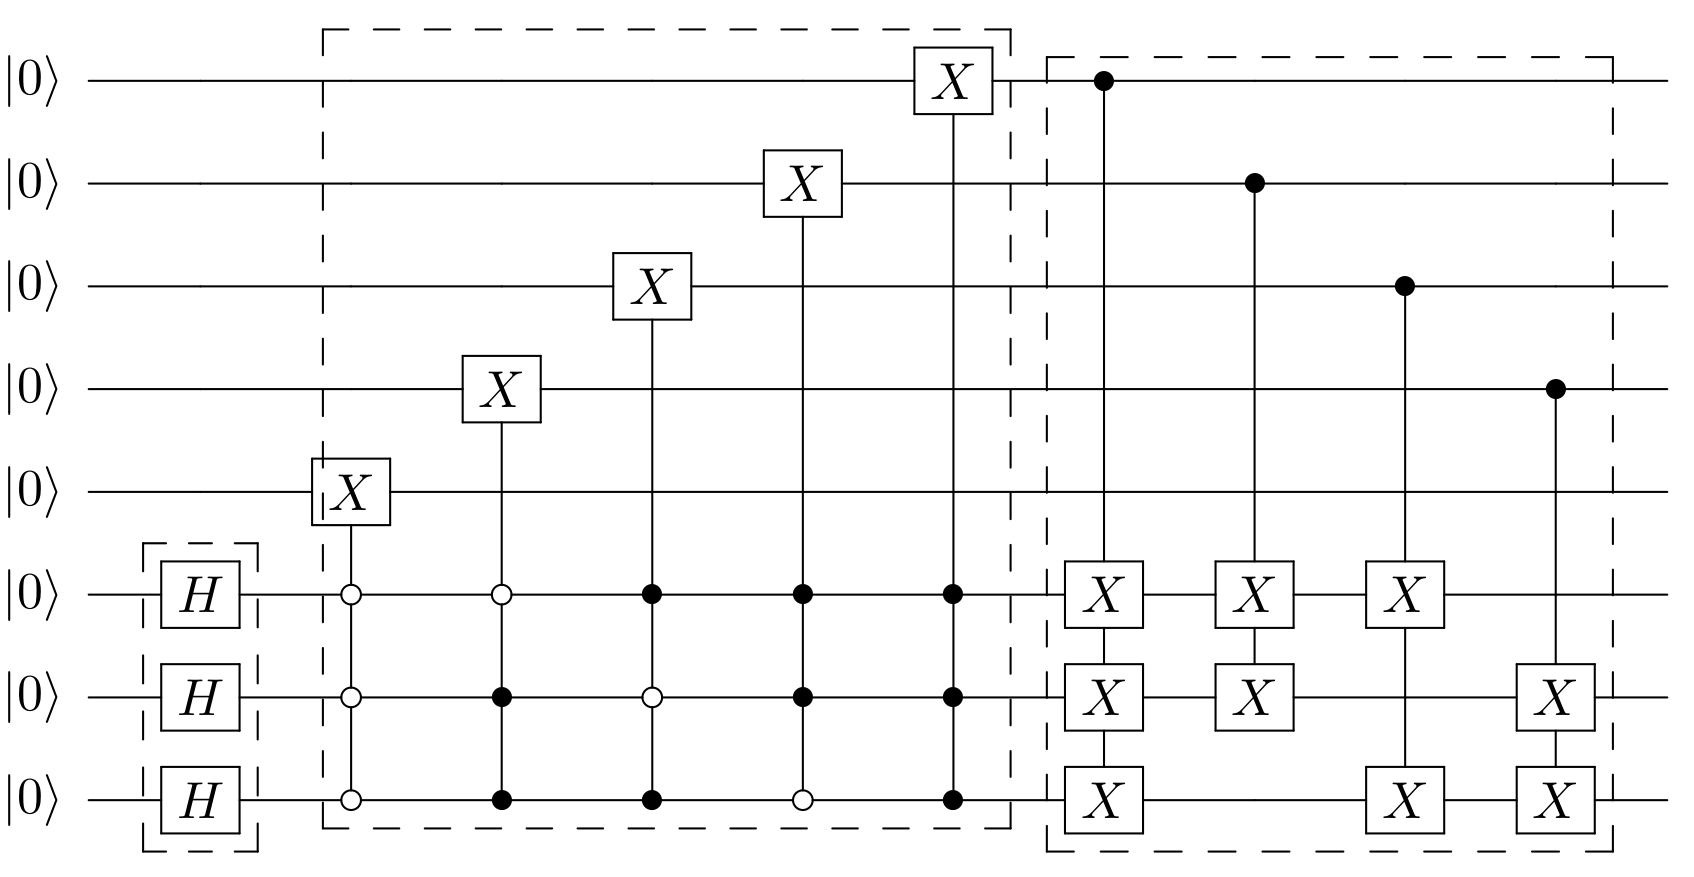
\includegraphics[width=0.8\linewidth]{pics/circuit-prepare-W-state-McClung.png}
\centering

\vspace{-.8em}

Circuit for computing the $\ket{W_8}$ state.

\vfill

\begin{theorem}[\cite{arunachalam2022parameterized}]
Any circuit which deterministically produces the
$\ket{W_n}$ state requires $\Omega(n)$ $T$ gates, unless ETH doesn't hold.
\end{theorem}

\vspace{-.5em}

\printbibliography[section=\therefsection]

\end{refsection}

\end{frame}





\begin{refsection}
\begin{frame}{\limdd Implementation}


\begin{exampleblock}{Circuit equivalence check implementation}
\begin{itemize}
	\item 	\limdd implemented in DDSIM~\cite{limdd2}.
	\item 	Tested on QFT, after random Clifford  circuit
\end{itemize}
\end{exampleblock}


\vspace{-.5em}

\centering
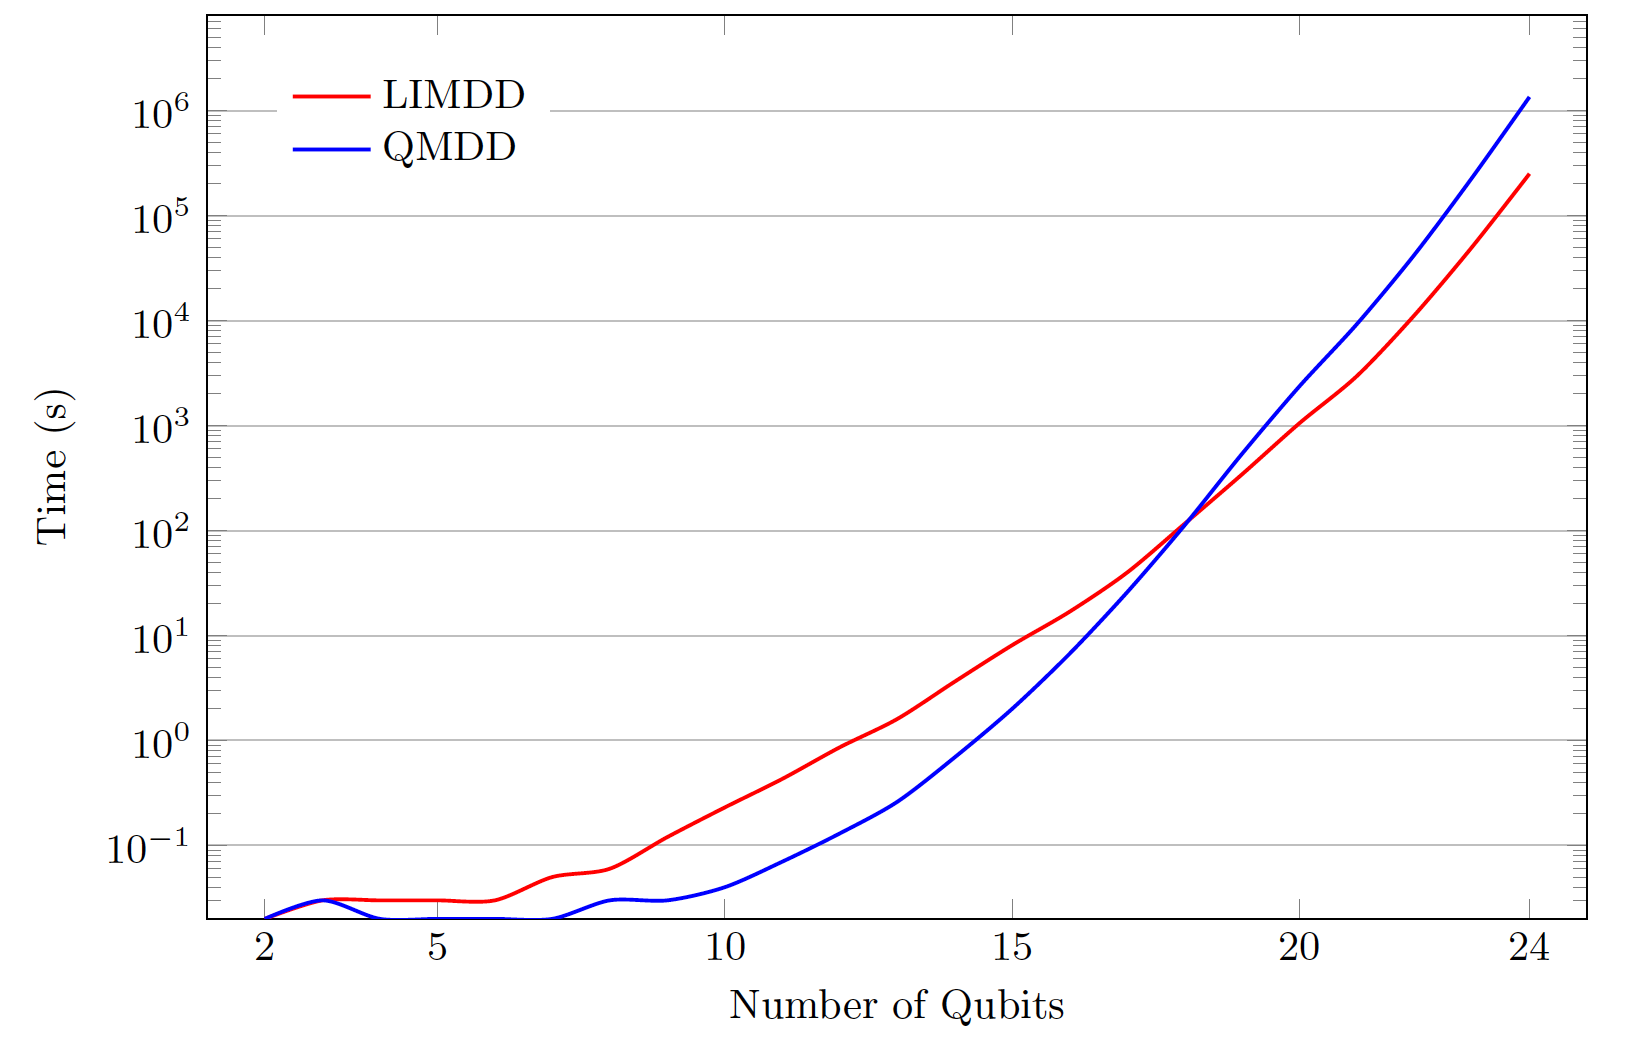
\includegraphics[height=5.cm]{plot.png}

\vspace{-.5em}

\centering
\printbibliography[section=\therefsection]
\vspace{-1em}
\url{https://github.com/cda-tum/mqt-limdd}

\end{frame}
\end{refsection}





\begin{refsection}
\begin{frame}{Other Variants of Algebraic Decision Diagrams}



\vspace{-.8em}

	
\begin{table}
\centering\footnotesize
\def\arraystretch{1.1}
\begin{tabular}{|p{5.5cm}|c|c|}
\hline
\textbf{(Quantum) decision diagrams}				& \textbf{Node merging strategy} &  \\\hline
Decision Tree	& (no merging) &  \\
\add~\cite{bahar1997algebric}, MTBDD~\cite{clarke1993spectral}, QuiDD~\cite{viamontes2003improving}			& $f = g$  &  \\
SLDD$_\times$~\cite{wilson2005decision,fargier2013semiring}, QMDD~\cite{miller2006qmdd}, TDD~\cite{hong2020tensor}	& $f = \gamma\cdot g$   & $\gamma \in \complex, \mathbb R, \dots$  \\
SLDD$_+$~\cite{fargier2013semiring}, EVBDD~\cite{lai1994evbdd}	& $f = g + \alpha$ & $\alpha \in \complex, \mathbb R, \dots$  \\
AADD~\cite{sanner2005AffineADDs}, FEVBDD~\cite{tafertshofer1997factored} 		& $f = \gamma\cdot g + \alpha$ & $\alpha,\gamma \in \complex, \mathbb R, \dots$ \\
\limdd~\cite{vinkhuijzen2021limdd}			& $f = \gamma  P_1\otimes \dots \otimes P_n \cdot g$ & $P_i \in \gen{\id, X,Y,Z}$   \\
\hline
\end{tabular}
\end{table}

\vspace{-.8em}


\nocite{limdd2}
\printbibliography[section=\therefsection]

\end{frame}
\end{refsection}



